\chapter{SIRE et LELA}\label{ch:sire-et-lela}

Les problématiques mises en jeu par l'énergie solaire sont nombreuses : intermittence, rendement, approvisionnement\ldots
Une question moins évidente à première vue posée par l'utilisation de ces technologies est celle de leur intégration à leur environnement.
En effet celle-ci diffère des modes de production classiques \textit{(les centrales thermiques et nucléaires sont en général très éloignés des populations)} en ce qu'elle est opérée au plus près des populations.
Il n'est alors pas rare de rencontrer des panneaux photovoltaïques dans la vie quotidienne : parkings, établissements publics et privés, et parfois les habitations elles-mêmes.
Ceci suppose un travail particulier à mener en parallèle de la conception des technologies, avec des compétences différentes.

C'est en sens qu'existe le \gls{SIRE}, qui vise à apporter au \gls{CEA} et au \gls{DTS} l'expertise nécessaire pour traiter ces problématiques.

\begin{figure}[H]
    \centering
    % Le contenu du diagramme est défini dans le fichier suivant
    \fbox{\begin{tikzpicture}[
    main/.style={text centered, text width=8cm, fill=green!20, draw, rectangle, rounded corners, font=\bfseries\Large},
    service/.style={text centered, text width=3cm, fill=gray!50, draw, rectangle, rounded corners},
    labo/.style={grow=down, xshift=4cm, text centered, text width=5cm, draw, rectangle, rounded corners, edge from parent path={(\tikzparentnode.225) |- (\tikzchildnode.west)}},
    first/.style    ={level distance=15ex},
    second/.style   ={level distance=30ex},
    third/.style    ={level distance=45ex},
    fourth/.style   ={level distance=60ex},
    fifth/.style    ={level distance=75ex},
    level 1/.style={sibling distance=12.5em, level distance=8em}]

    \node[main, anchor=south]{Département des Technologies Solaires}
    [edge from parent fork down]
    %
    child{node (d1) [service] {\textbf Service \\ Procédés \\ et \textbf Cellules \textbf Photo\textbf{v}oltaïques}}
    %
    child{node (d2) [service] {\textbf Service \textbf Modules \\ et \textbf Systèmes \textbf Photovoltaïques}
        child[labo,first]  {node {\textbf Laboratoire \\ de \textbf Stockage \textbf Stationnaire \\pour \textbf Applications ENR}}
        child[labo,second] {node {\textbf Laboratoire \\ d'\textbf Intégration \textbf Énergétique Locale \\et \textbf Autoconsommation}}
        child[labo,third]  {node {\textbf Laboratoire \\ de Pilotage \textbf Intelligent \\ des \textbf Réseaux \textbf Électriques}}
    }
    %
    child{node (d3) [service] {\textbf Service \\ \textbf Modules \\ \textbf Systèmes \textbf Photovoltaïques}};
\end{tikzpicture}}
    \caption{Organigramme simplifié de la DTS et du SIRE}
    \label{fig:organigramme-DTS}
\end{figure}

\newpage Au sein du service, le \gls{LELA} travaille spécifiquement sur la consommation énergétique des bâtiments, notamment pour apporter une vision prospective sur les conséquences de l'équipement de bâtiments en panneaux solaires.
À cet égard, son activité est représentative du \gls{CEA} : les échelles des parcs de bâtiments étudiés sont locales \textit{(quartier Cambridge à Grenoble, étudié dans le cadre de cette alternance)}, nationales, européennes et mondiales\footnote{ces derniers projets, encore en cours n'étant pas mentionnés ici pour des raisons de confidentialité}

La trentaine de membres du laboratoire \textit{(ingénieurs chercheurs, techniciens et doctorants)} s'appuient sur des simulations numériques et sur des expérimentations à échelle réelle, en particulier par l'utilisation active d'une des trois plateformes d'équipements de l'\gls{INES}, dont on peut voir une partie sur les photos ci-dessous, montrant les maisons \gls{INCAS}, inhabitées car spécialement dédiées aux travaux de recherche en énergétique du bâtiment.

\begin{figure}[H]
    \centering
        \subfloat[Vue extérieure \textit{(Crédit photo : Patrick Avavian)}]{\fbox{
            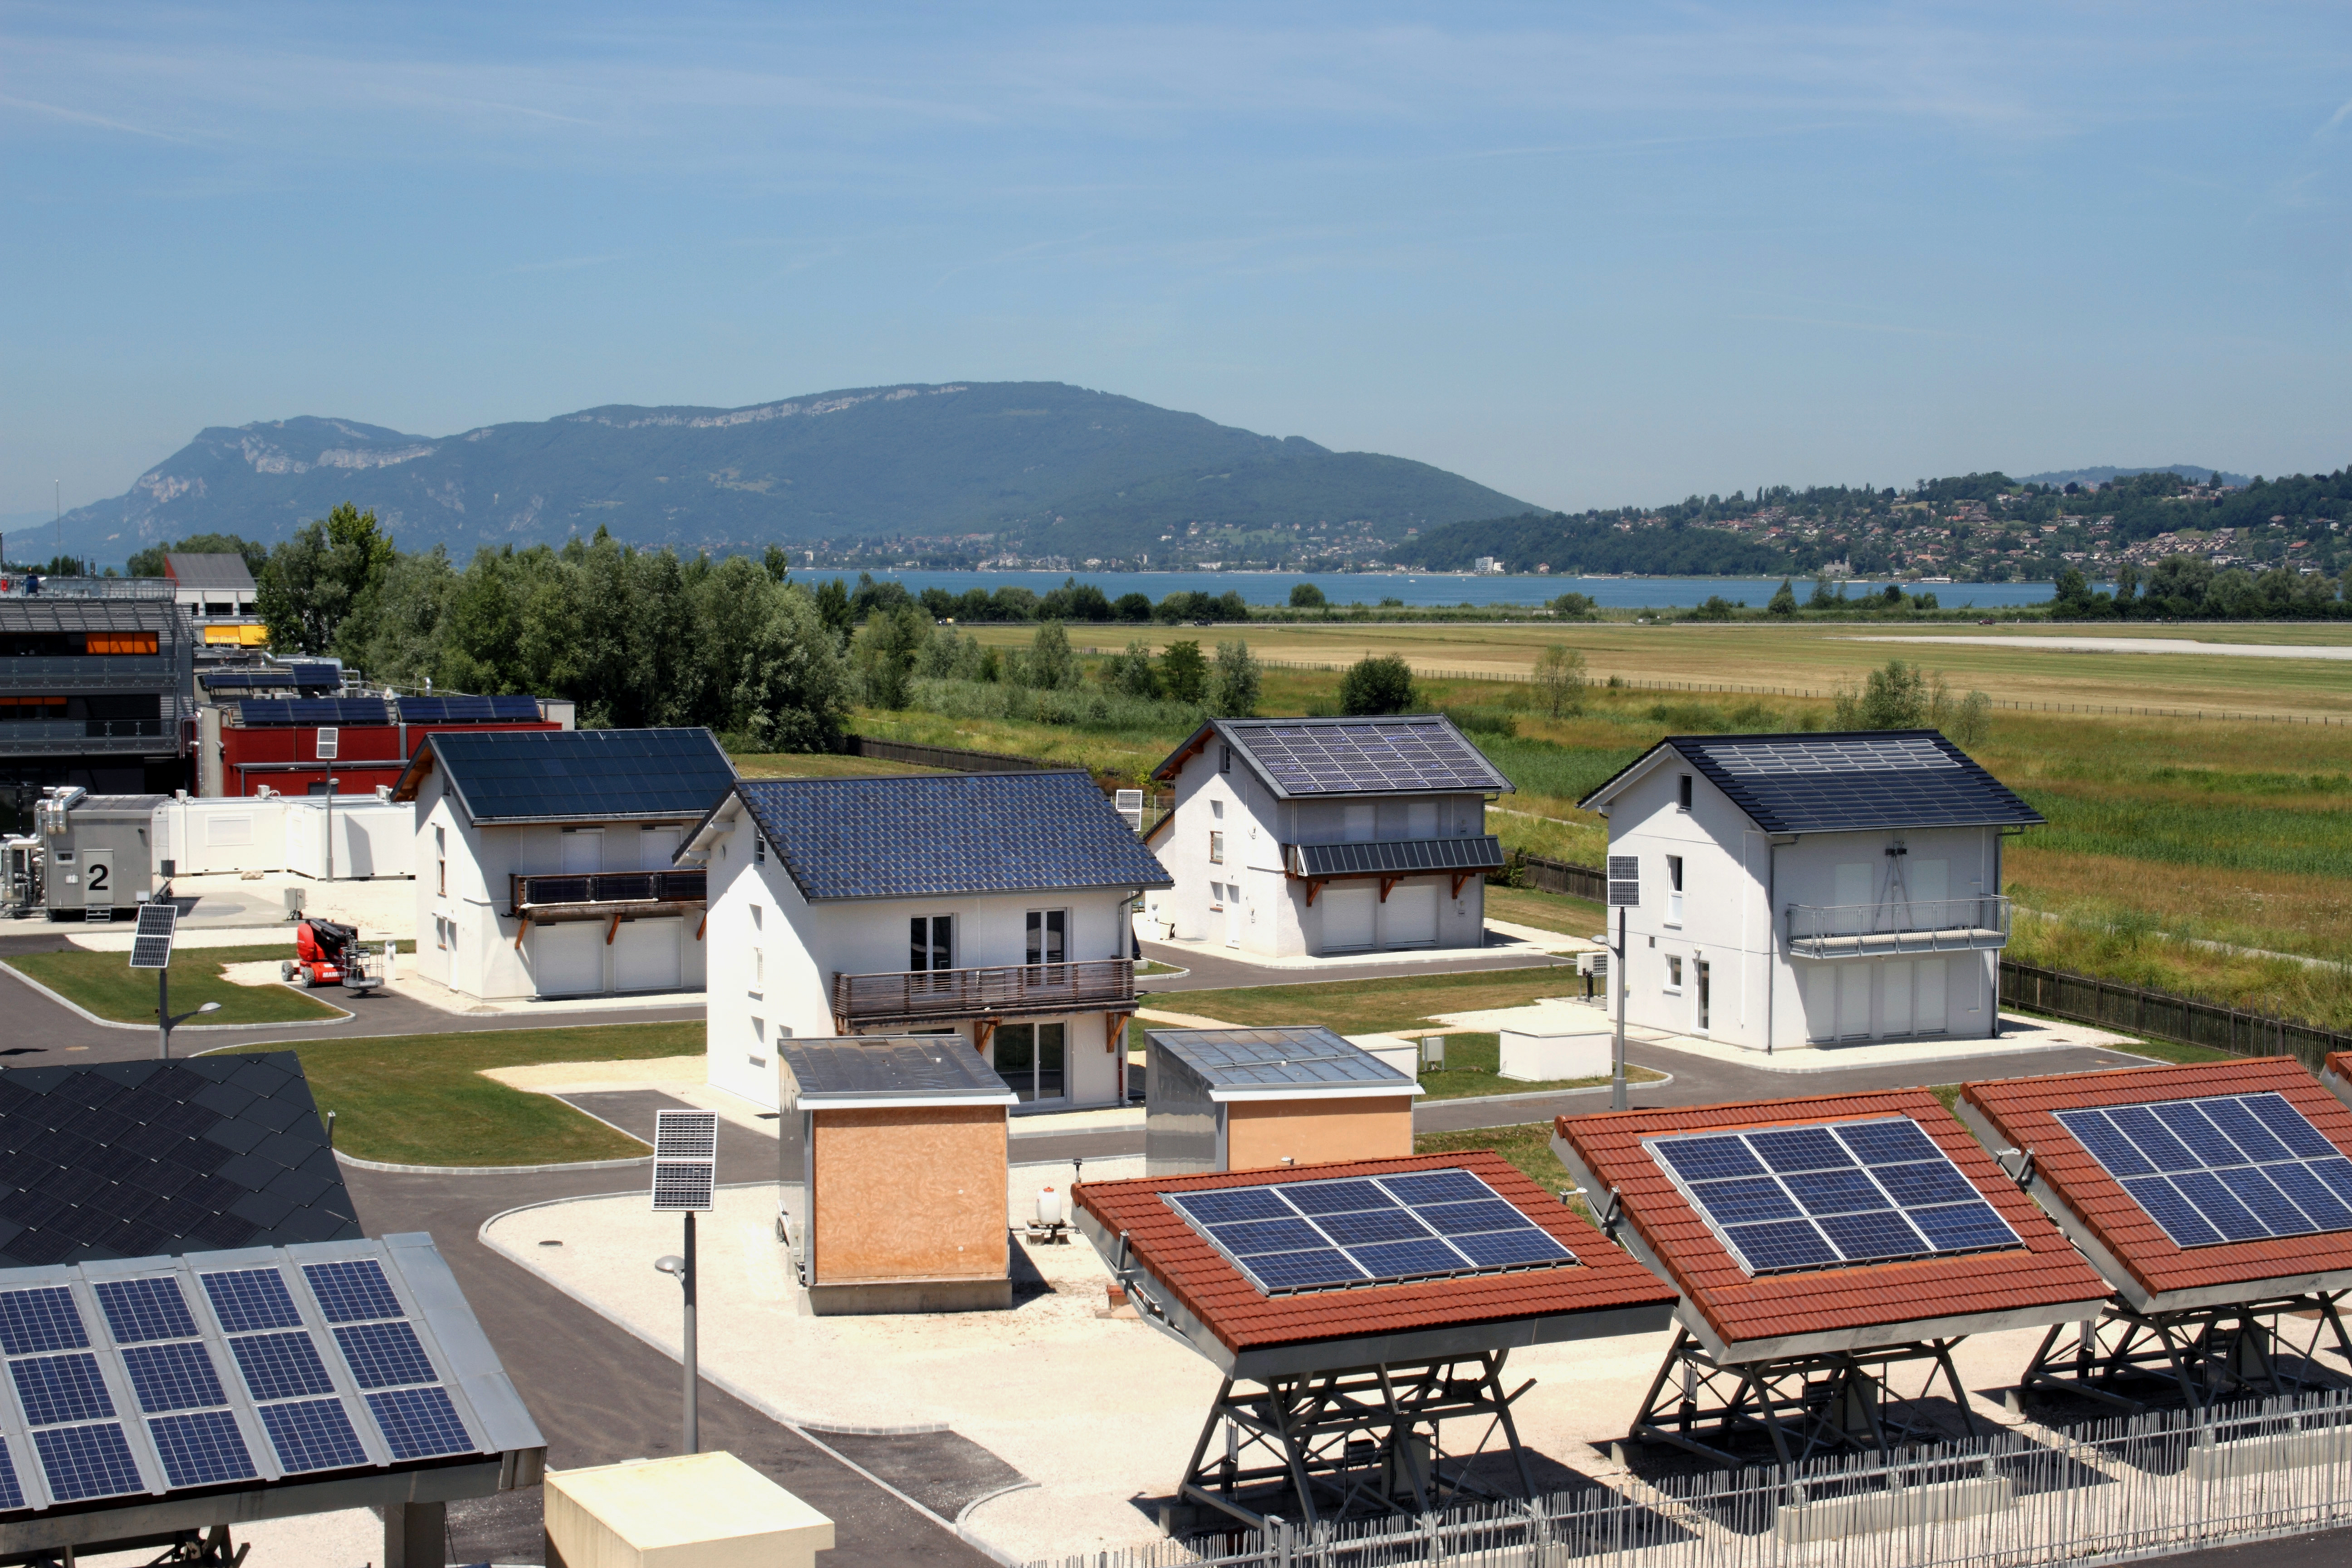
\includegraphics[width = 0.75\textwidth]{figures/illustrations/photos/INCA_Patrick AVAVIAN}}}\\
        \subfloat[Capteurs installés pour mesurer les fuites d'air vers l'extérieur \textit{(Crédit photo : Gilles Rolles)}]{\fbox{
            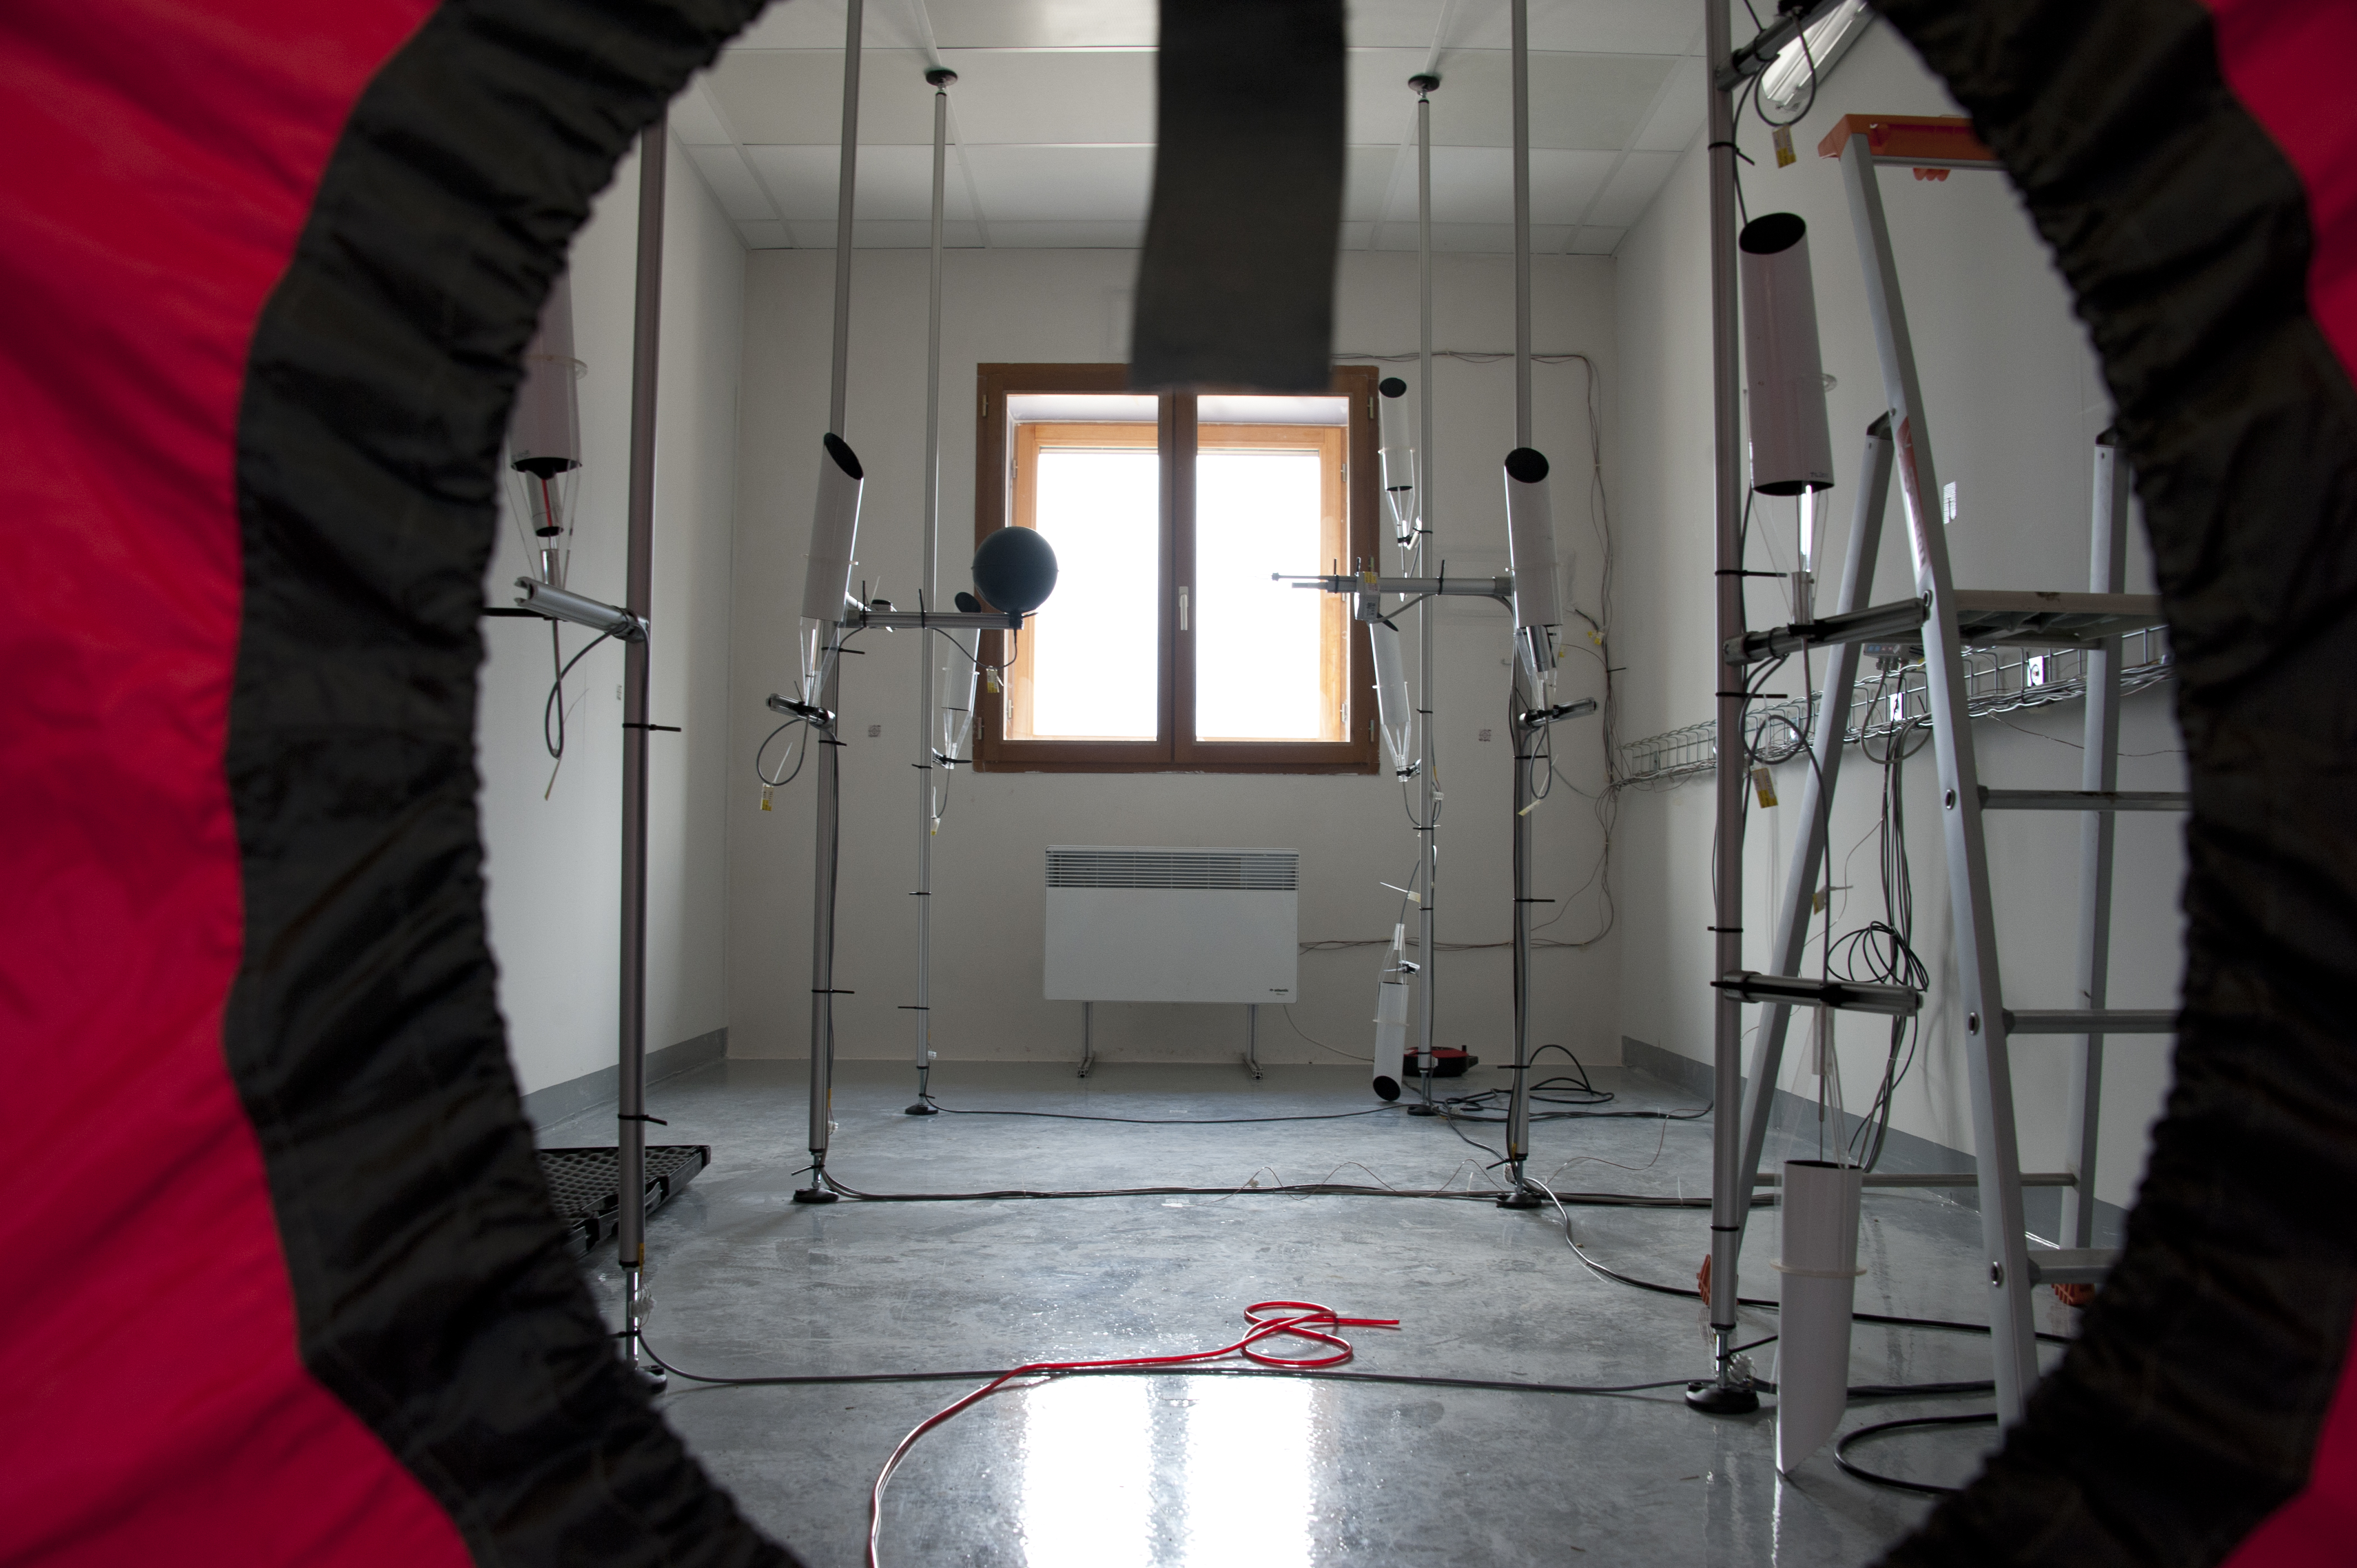
\includegraphics[width = 0.75\textwidth]{figures/illustrations/photos/INCA_int_Gilles_ROLLES}}}
    \caption{Maisons INCAS du LELA}\label{fig:figure}
\end{figure}
